\documentclass[a4paper,10pt]{article}
%\usepackage[latin1]{inputenc} % Paquetes de idioma (otro encoding)
\usepackage[utf8]{inputenc} % Paquetes de idioma
\usepackage[spanish]{babel} % Paquetes de idioma
\usepackage{graphicx} % Paquete para ingresar gráficos
\usepackage{grffile}
\usepackage{hyperref}
\usepackage{fancybox}
\usepackage{amsmath}
\usepackage{amsfonts}
\usepackage{listings}
\usepackage{pdfpages}
% Paquetes de macros de Circuitos
%\usepackage{pstricks}
\usepackage{tikz}

% Encabezado y Pié de página
% Paquete para encabezados y pie de página
\usepackage{fancyhdr} 
% Sin esta línea no se imprimiría el encabezado en todas las páginas
\pagestyle{fancy} 

% Borra el encabezado anterior (Por defecto escribe el título de la 
%  sección en la que se encuentra la hoja
\fancyhf{} 
\setlength{\headheight}{22.55pt}
\fancyhead[L]{
	{\textsf{Facultad de Ingenieríaa $-$ Universidad de Buenos Aires 
    \\ 75.61 Taller de Programación III}}
}
%\addtocounter{page}{5}
\fancyhead[R]{\thepage}

% Ajusta el tamaño de las líneas separadoras en el pié de página
\renewcommand{\footrulewidth}{0.4pt}
 % Ajusta el tamaño de las líneas separadoras en el encabezado
\renewcommand{\headrulewidth}{0.4pt} 

\fancyfoot[L]{
	{\textsf{TP N$^{\circ}$2 - Ejercicio de Colas (RabbitMQ)} \\
	{\textsf{Integrantes: Torres Feyuk}}
	}
}
		

% Carátula del Trabajo
\title{ \author{} % Lo pongo para que el warning no moleste :p
\setlength{\unitlength}{1cm} %  Especifica la unidad de trabajo
\thispagestyle{empty}

\begin{picture}(18,0)
\put(0,0){
\includegraphics[width=1.5cm, height=3cm]{Imagenes/Logo1.png}}

\put(10.5,0){
\includegraphics[width=3cm, height=3cm]{Imagenes/Logo2.png}}

\end{picture}
\\[1.5cm]
\begin{center}
	\textbf{{\Huge Facultad de Ingeniería \\ Universidad de Buenos Aires}}
    \\[2cm]
	{75.61 Taller de Programación III}\\[0.5cm]
	{TP N$^{\circ}$2 - Ejercicio de Colas (RabbitMQ)}\\[2.5cm]
\end{center}

\begin{flushleft}
	\textbf{Profesor: Andrés Veiga} \\
    \textbf{JTP: Pablo Roca} \\[1cm]
	\textbf{Integrantes:} \\[1cm]

	\begin{tabular}{|c|c|c|}
		\hline
		\textbf{\normalsize Padrón} & \textbf{\normalsize Nombre} 
                                    & \textbf{\normalsize Email} \\
		\hline
		\normalsize 89579 & \normalsize Torres Feyuk, Nicolás R. Ezequiel 
                          & \normalsize ezequiel.torresfeyuk@gmail.com \\
		\hline
	\end{tabular}
\end{flushleft}
\date{} % Hace que no se imprima la fecha en la cual se compilo el .tex
 }

\begin{document}
	\maketitle % Hace que el título anterior sea el principal del documento
	\newpage

    % Esta línea genera un indice a partir de las secciones y 
    % subsecciones creadas en el documento
	\tableofcontents 
	\newpage

	\section{Introducción}
		El presente trabajo práctico consiste en diseñar e 
        implementar un sistema de recepción de pedidos masivos. Para 
        realizar esta tarea, se deben implementar procesos que
        modelen diferentes partes/tareas del sistema. Para comunicar los 
        procesos, se deben utilizar cola de mensajes distribuidas. \\
        \indent RabbitMQ es un middleware orientado a mensajes el cual 
        permite conectar diferentes procesos a través de colas de mensajes
        distribuídas. El objetivo del presente trabajo consiste en:
        
        \begin{itemize}
            \item Focalizar el desarrollo de sistema en la recepción fluída
            de \textbf{Orders} y \textbf{Queries} realizadas por los clientes
            \item Comprender el funcionamiento básico de RabbitMQ 
            \item Paralelizar la mayor cantidad de tareas posible, exprimiendo
            en el máximo nivel posible el middleware de colas a utilizar
            \item Crear y diseñar una arquitectura escalable horizontalmente
            de forma de responder de forma eficaz y eficiente ante nuevos
            requerimientos
        \end{itemize}

    \newpage
    \section{Arquitectura 4 + 1}
    \subsection{Casos de Uso}
        En la figura \ref{DiagCU} se exhibe el diagrama de casos de uso del 
        sistema. Se detalla a continuación cada uno de las entradas del mismo:
        \begin{itemize}
            \item \textbf{Enviar Orden:} El cliente envía una orden de compra,
            la cual contiene un identificador único de la orden más la cantidad
            que desea obtener un determinado producto. Por el momento el 
            sistema no acepta más de un producto por orden.
            \item \textbf{Consultar Orden:} Un cliente consulta en que 
            estado se encuentra su orden. El sistema puede responderle con 
            alguno de los siguientes estados: 
            \begin{itemize}
                \item \textit{RECEIVED}
                \item \textit{ACCEPTED}
                \item \textit{REJECTED}
                \item \textit{DELIVERED}
            \end{itemize}
            \item \textbf{Procesar Orden:} Como se considera a los Empleados
            externos al sistema, el procesamiento de una orden es válido como
            caso de uso. Los empleados obtienen los pedidos a procesar 
            (aquellos que fueron aceptados), y al terminar de trabajar con los
            mismo proceden a cambiar su estado a \textit{DELIVERED}
            \item \textbf{Incrementar Stock:} Un proveedor se encarga de 
            aumentar el stock de los productos ofrecidos por la aplicación
        \end{itemize}

        \begin{figure}[!htb]                                             
            \centering                                                   
            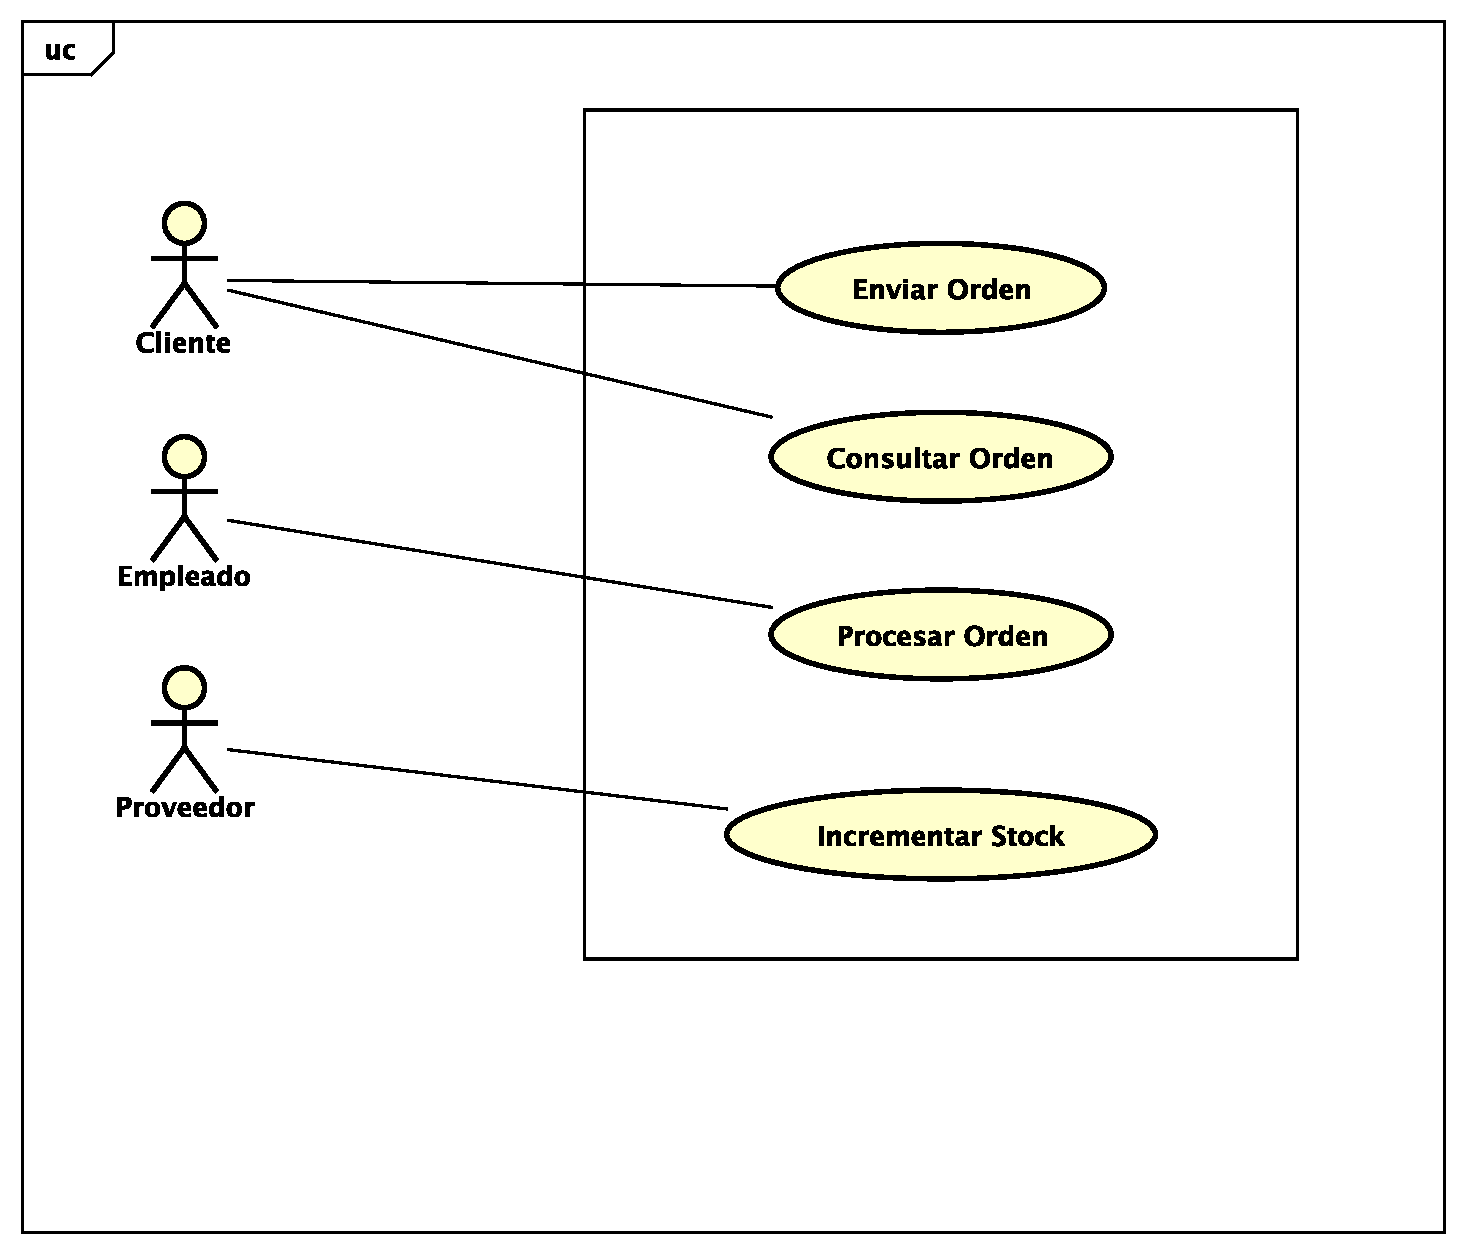
\includegraphics[width=8cm,origin=c]{Imagenes/Casos_De_Uso.pdf}        
            \caption{Diagrama de Casos de Uso} \label{DiagCU}
        \end{figure}

    \newpage
    \subsection{Vista Lógica}
        \begin{figure}[!htb]                                             
            \centering                                                   
            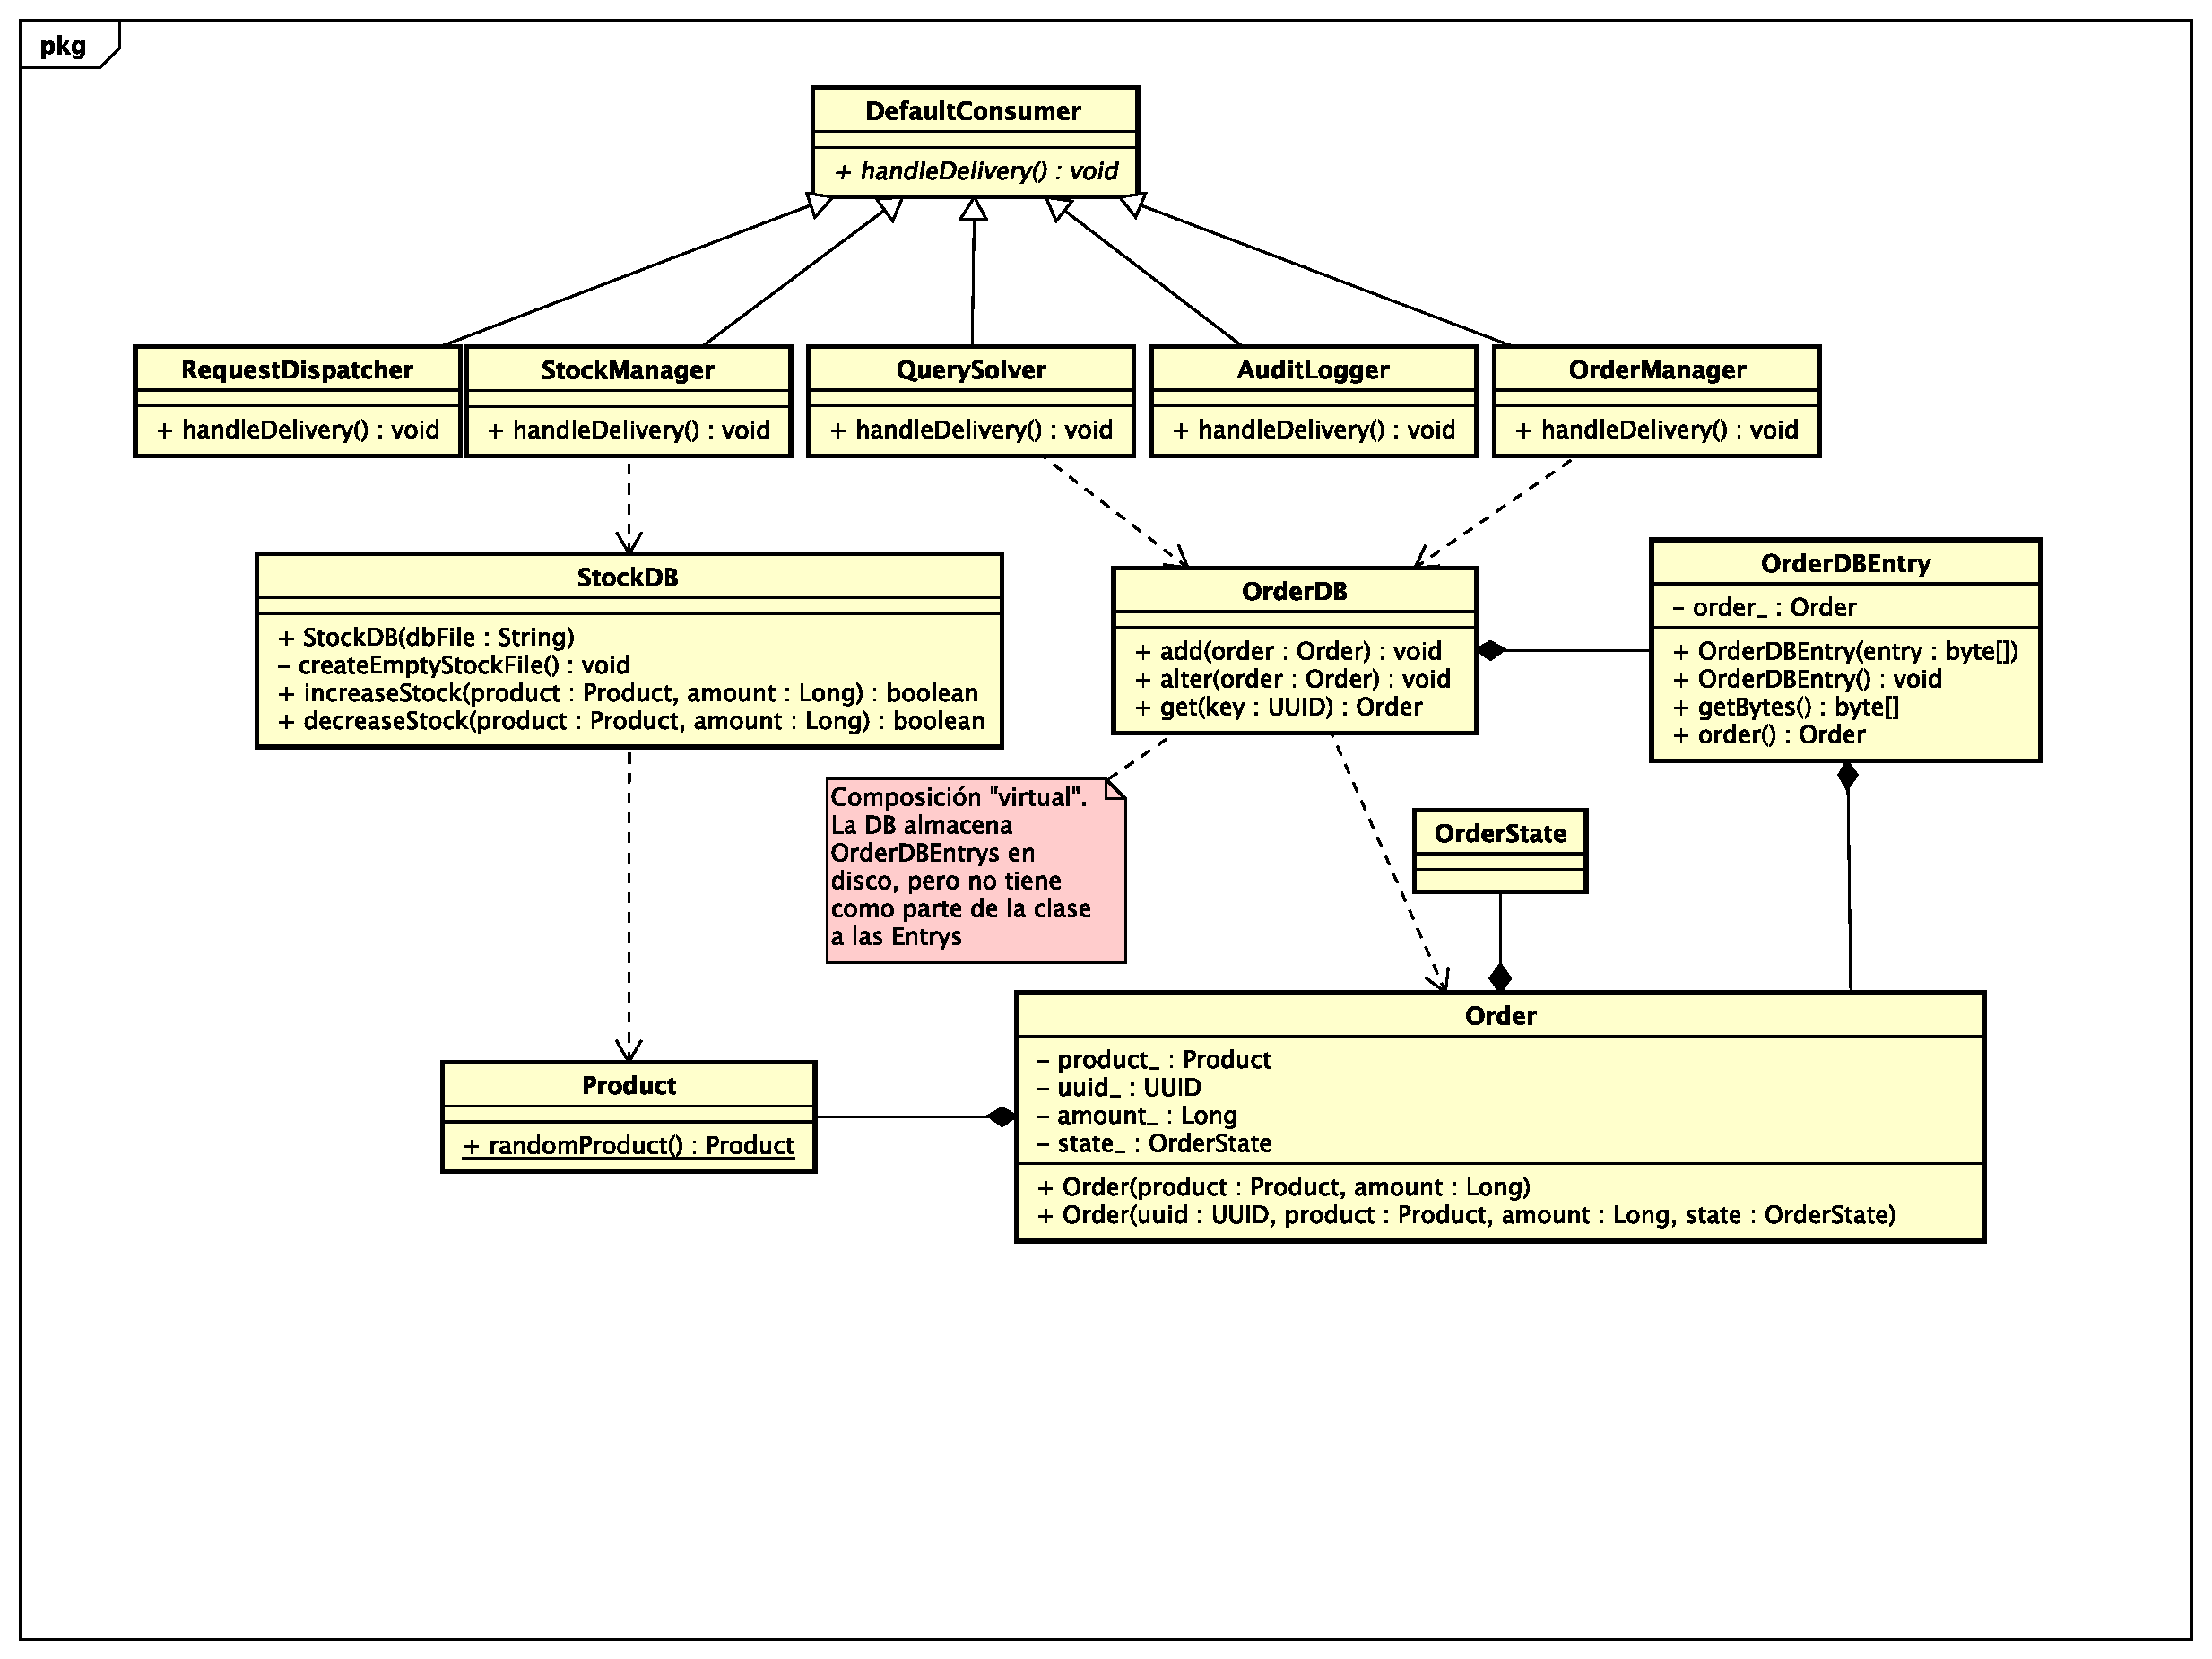
\includegraphics[width=18cm,angle=90,origin=c]{Imagenes/Diagrama_Clases.pdf} 
            \caption{Diagrama de Clases} \label{DiagClases}
        \end{figure}

    \newpage
    \subsection{Vista de Despliegue}
        Para la vista de despliegue se decidió realizar un diagrama de 
        robustez y un diagrama de despliegue. El primero explica como los 
        diferentes procesos del sistema se comunican entre sí a través de 
        diferentes colas de mensaje, mientras que el segundo intenta representar
        la arquitectura física de la aplicación.
        
        \subsubsection{Diagrama de Robustez}
        El mismo se puede visualizar en la figura \ref{DiagRobustez}. Debido 
        a que no se encontro una herramienta adecuada para graficar el mismo,
        se detalla a continuación los elementos utilizados junto con el
        significado de cada uno:

        \begin{figure}[!htb]                                             
            \centering                                                   
            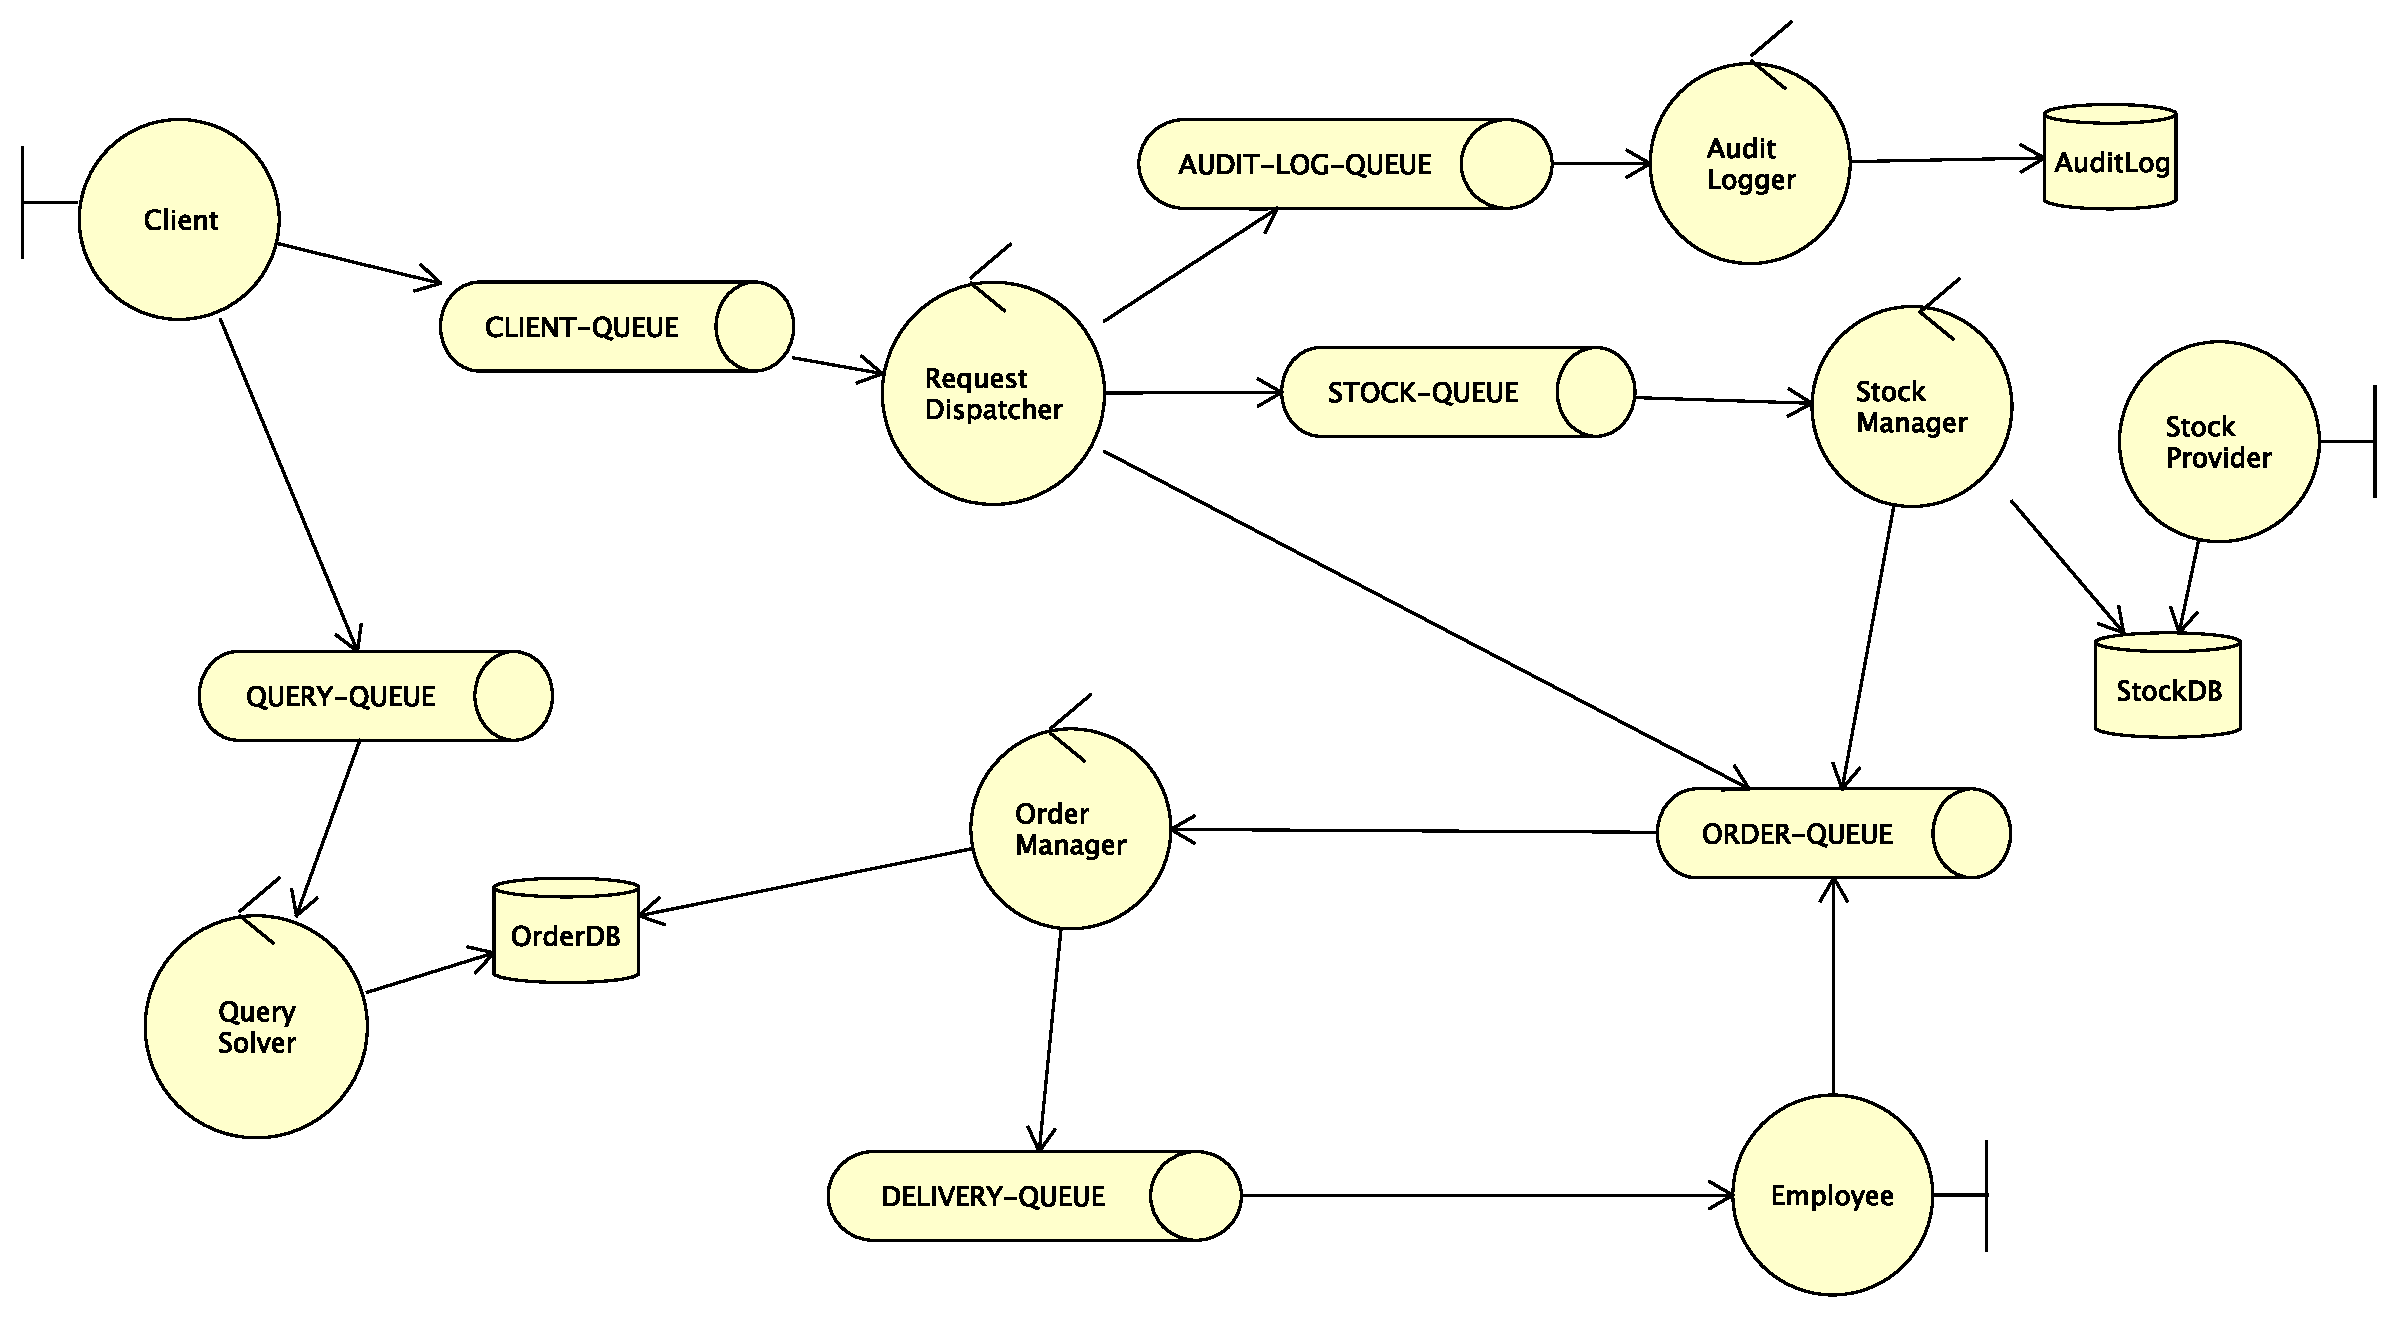
\includegraphics[width=20cm,angle=90,origin=c]{Imagenes/robustez.pdf}        
            \caption{Diagrama de Robustez} \label{DiagRobustez}
        \end{figure}

        \begin{itemize}
            \item \textbf{Círculos Rojos:} Procesos que envían estímulos al 
            sistema
            \item \textbf{Círculos Verdes:} Controladores. Puede haber N 
            de ellos          
            \item \textbf{Círculos Amarillos:} Controladores. Por cuestiones
            de modelo de negocio, solo puede haber uno de estos controladores
            de cada tipo al mismo tiempo
            \item \textbf{Colas:} RabbitMQ Queues. Las flechas entrantes        
            indican que un controlador ingresa mensajes en la cola. Flechas
            salientes indican que un controlador saca elementos de la cola.
            \item \textbf{Discos:} Archivos físicos los cuales, en el presente
            trabajo, simulan el funcionamiento de bases de datos relacionales.
        \end{itemize}

        \subsubsection{Diagrama de Despliegue}
        El diagrama se despliegue se exhibe en la figura \ref{DiagDespl}. Cada 
        nodo representa a un servidor físico independiente, el cual corre 
        aplicaciones y puede o no tener Base de Datos. Se procede a detallar
        cada uno de los nodos:

        \begin{itemize}
            \item \textbf{DispathServer:} En este nodo corren los procesos
            RequestDispatcher que se encargar de recibir las \textbf{Orders}
            de los clientes para derivarlas a otros nodos. En el diagrama
            se puede ver que existen dos nodos de este tipo. Con esto se 
            quiere representar que se puede escalar este nodo agregando
            N de los mismos de forma transparante al sistema.
            \item \textbf{AuditLogServer:} Nodo donde se encuentra el log 
            de auditoría. Como los logs deben ser almacenados en orden, 
            solo puede haber un proceso corriendo de este tipo. El proceso
            debe correr en un servidor aparte debido a que este es un punto
            sensible del sistema y debe ser optimizado en la mayor medida
            posible.
            \item \textbf{StockServer:} En el presente nodo se encuentra 
            la base de datos en donde se almacena el Stock de los productos.
            En el nodo se pueden ver más de una aplicación, lo cual indica
            que se pueden correr N instancias de este proceso en el dispositivo
            físico, pero que no se puede agregar más nodos de este tipo. Esto
            último se debe a que los procesos a través de I/O syscalls a la 
            DB las cuales deben correrse en el mismo servidor físico donde
            se encuentra la DB en cuestión.
            \item \textbf{OrderServer:} En el presente nodo se encuentran los
            procesos OrderManager y QuerySolver. Se cumplen los mismos 
            requisitos que para el proceso StockManager, dado que estos 
            procesos también realizando un acceso físico a un DB (OrderDB).
           
        \end{itemize}


        \begin{figure}[!htb]                                             
            \centering                                                   
            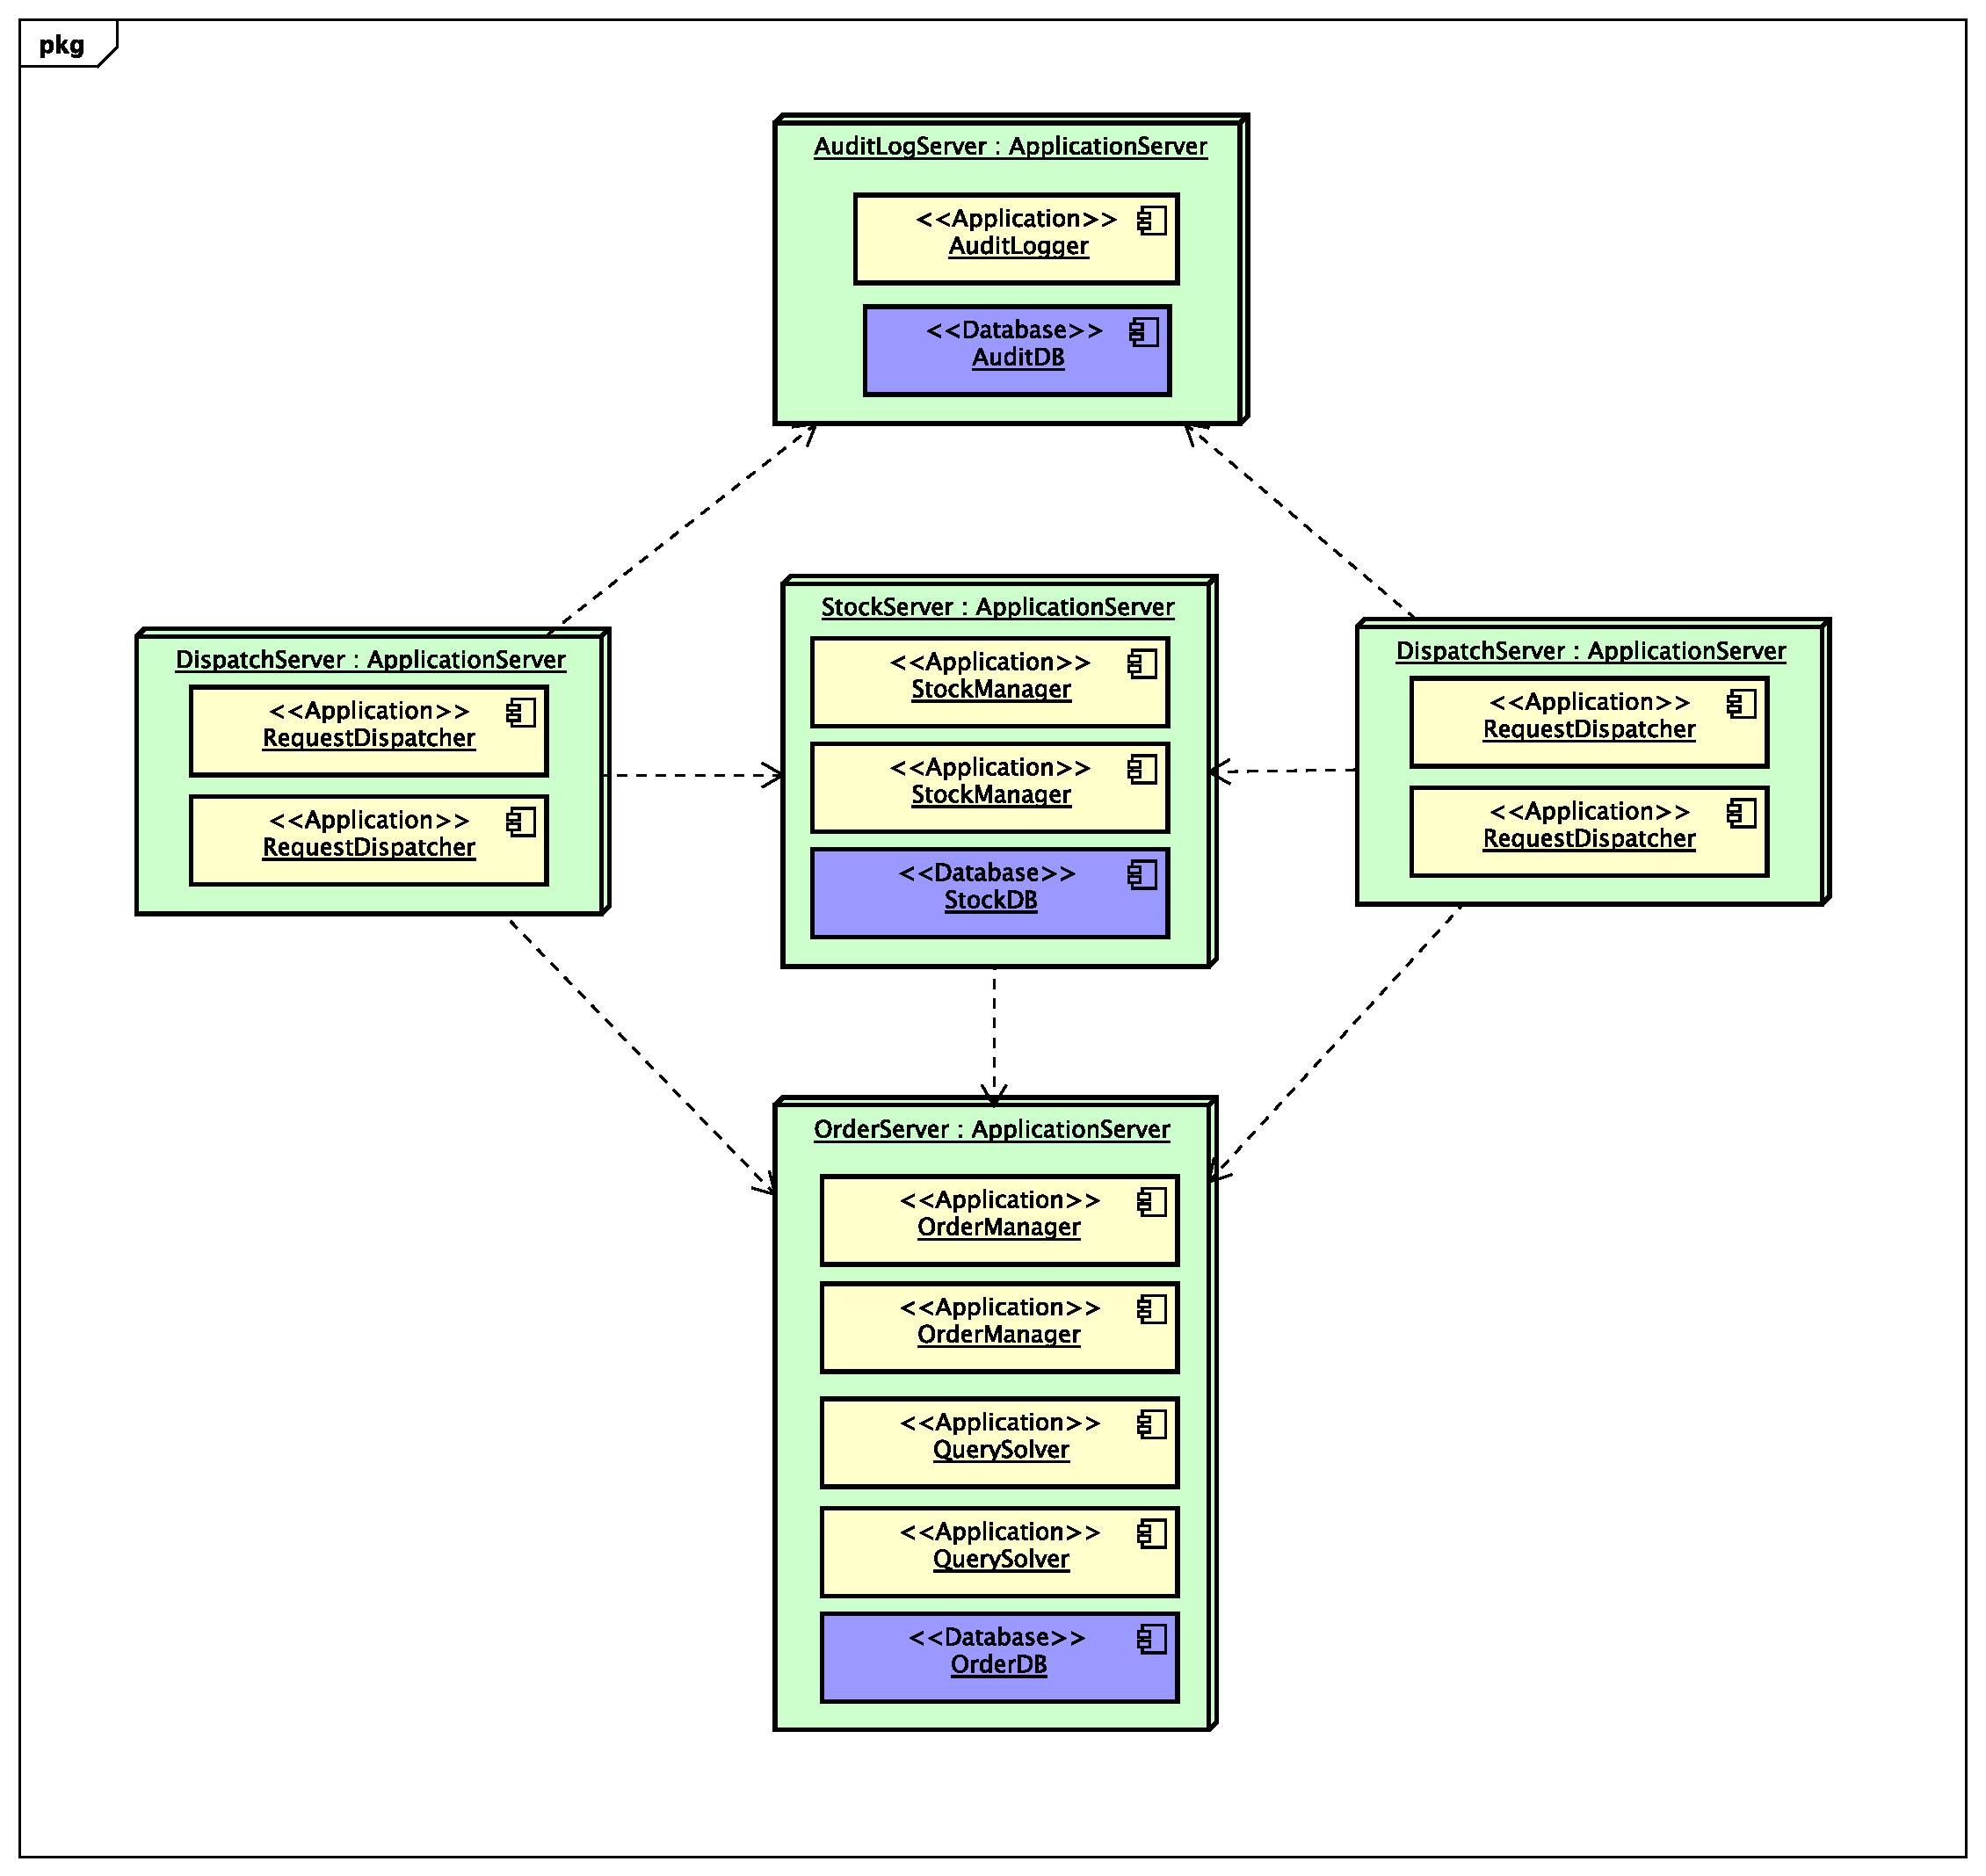
\includegraphics[width=15cm,origin=c]{Imagenes/Despliegue.pdf}        
            \caption{Diagrama de Despliegue} \label{DiagRobustez}
        \end{figure}
   
    %\newpage 
    %\section{Código}
    %    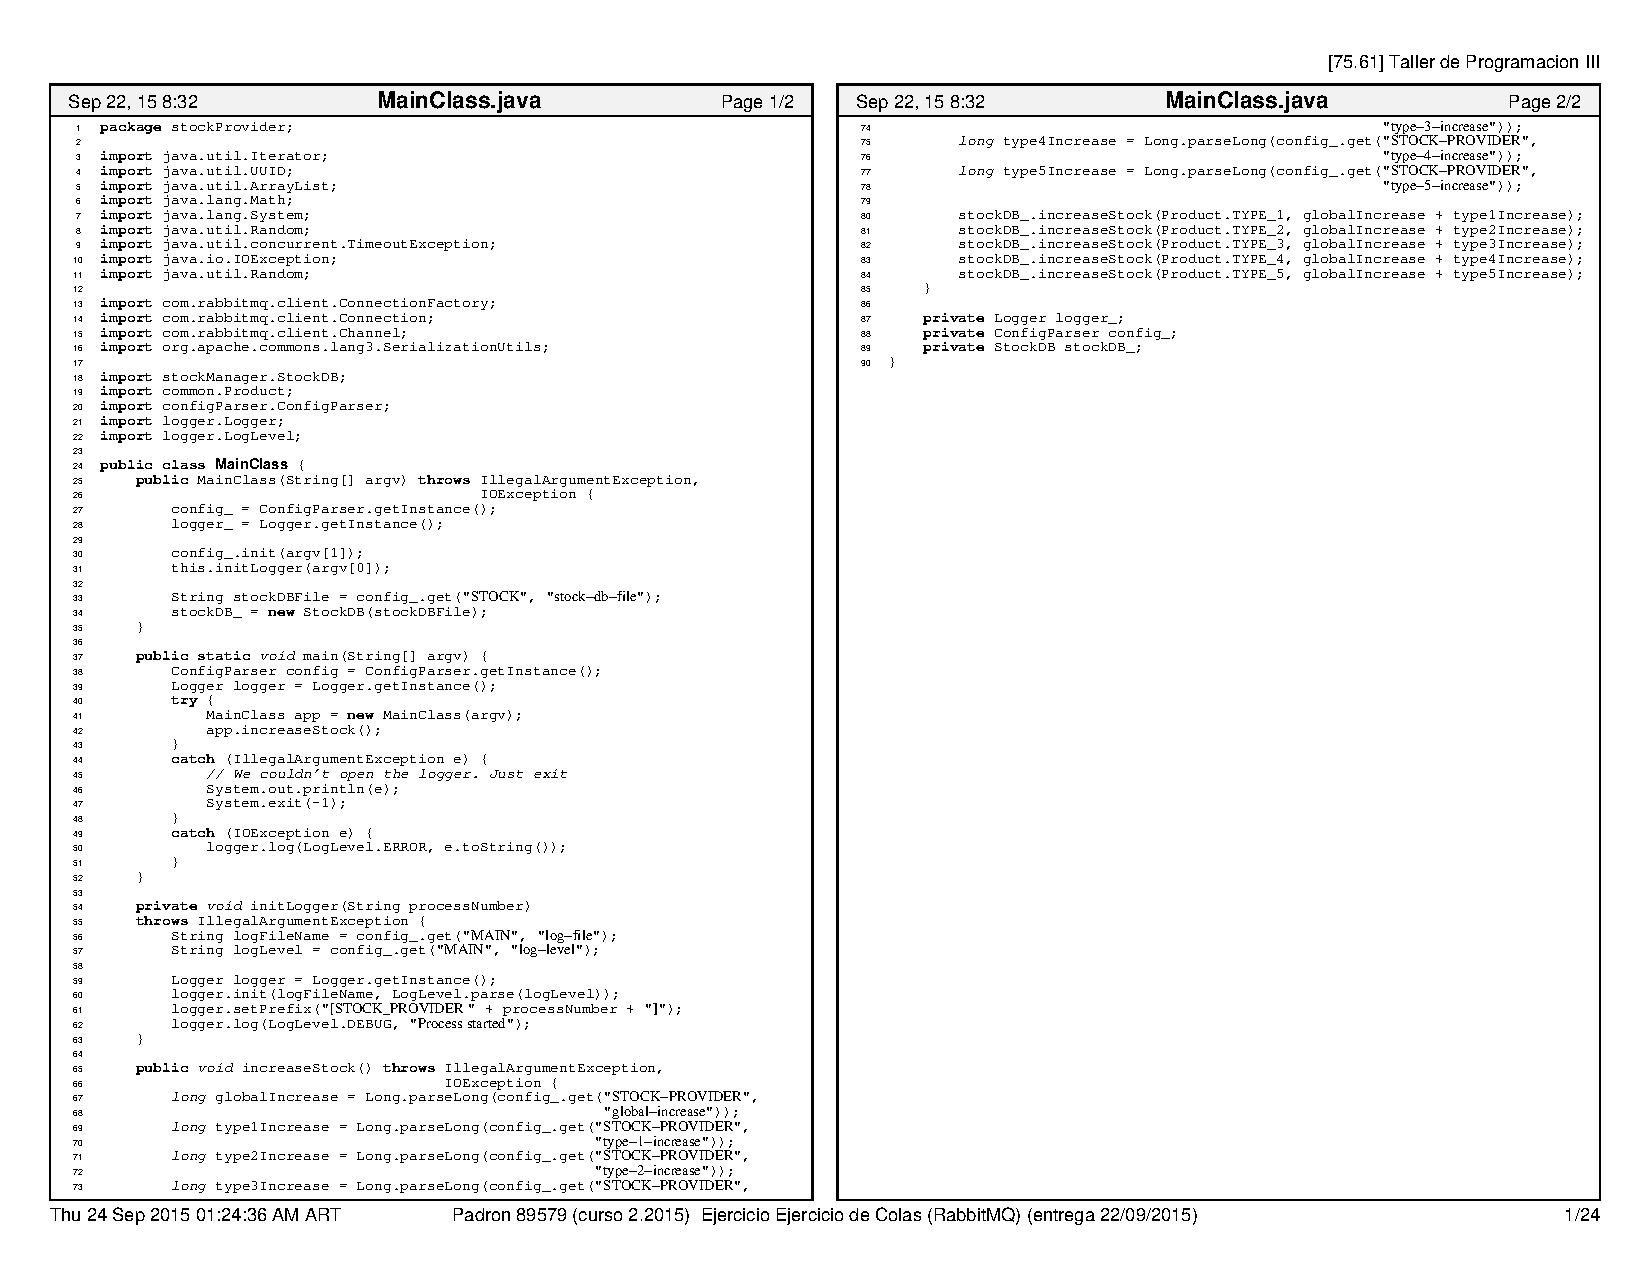
\includepdf[pages=-,scale=.80,pagecommand={},landscape=true]{codigo.pdf}
\end{document}

